% ------------------------------------------------------------------------------
% OpenQuake-engine Users Manual
% 
% Authors: 
% 	H. Crowley 		- Executive Committee - GEM Foundation, Pavia, Italy
% 	D. Monelli 		- GEM Model Facility, Zurich, Switzerland
% 	M. Pagani 		- Executive Committee - GEM Foundation, Pavia, Italy
% 	V. Silva 		- GEM Model Facility, Pavia, Italy
%	G. Weatherhill 	- GEM Model Facility, Pavia, Italy
% 
% Document distributed under the Common Creative License 
% © GEM Foundation, Pavia, February 2013
% ------------------------------------------------------------------------------
\documentclass[12pt,a4paper,headings=small,version=last,dvips]{scrbook}
%\documentclass[12pt,a4paper,headings=small,version=first,dvips]{scrbook}
% --------------------------------------------------------------------- Packages
%%%%%%%%%%%%%%%%%%%%%%%%%%%%%%%%%%%%%%%%%
% The Legrand Orange Book
% LaTeX Template
% Version 1.4 (12/4/14)
%
% This template has been downloaded from:
% http://www.LaTeXTemplates.com
%
% Original author:
% Mathias Legrand (legrand.mathias@gmail.com)
%
% License:
% CC BY-NC-SA 3.0 (http://creativecommons.org/licenses/by-nc-sa/3.0/)
%
% Compiling this template:
% This template uses biber for its bibliography and makeindex for its index.
% When you first open the template, compile it from the command line with the 
% commands below to make sure your LaTeX distribution is configured correctly:
%
% 1) pdflatex rmtk-docs
% 1a) pdflatex -shell-escape rmtk-docs
% 2) makeindex rmtk-docs.idx -s StyleInd.ist
% 3) biber rmtk-docs
% 4  makeglossaries rmtk-docs
% 4) pdflatex rmtk-docs x 2
%
% After this, when you wish to update the bibliography/index use the appropriate
% command above and make sure to compile with pdflatex several times 
% afterwards to propagate your changes to the document.
%
% This template also uses a number of packages which may need to be
% updated to the newest versions for the template to compile. It is strongly
% recommended you update your LaTeX distribution if you have any
% compilation errors.
%
% Important note:
% Chapter heading images should have a 2:1 width:height ratio,
% e.g. 920px width and 460px height.
%
%%%%%%%%%%%%%%%%%%%%%%%%%%%%%%%%%%%%%%%%%

%----------------------------------------------------------------------------------------
%	PACKAGES AND OTHER DOCUMENT CONFIGURATIONS
%----------------------------------------------------------------------------------------

\documentclass[11pt,fleqn]{book} % Default font size and left-justified equations

\usepackage[top=3cm,bottom=3cm,left=3.2cm,right=3.2cm,headsep=10pt,a4paper]{geometry} % Page margins

\usepackage{xcolor} % Required for specifying colors by name
\definecolor{ocre}{RGB}{243,102,25} % Define the orange color used for highlighting throughout the book

% Font Settings
\usepackage{avant} % Use the Avantgarde font for headings
%\usepackage{times} % Use the Times font for headings
\usepackage{mathptmx} % Use the Adobe Times Roman as the default text font together with math symbols from the Sym­bol, Chancery and Com­puter Modern fonts

\usepackage{microtype} % Slightly tweak font spacing for aesthetics
\usepackage[utf8]{inputenc} % Required for including letters with accents
\usepackage[T1]{fontenc} % Use 8-bit encoding that has 256 glyphs

% Bibliography
\usepackage{csquotes}
\usepackage[style=alphabetic,
            sorting=nyt,
            sortcites=true,
            natbib=true,
            style=authoryear,
            maxcitenames=2,
            maxbibnames=100,
            autopunct=true,
            babel=hyphen,
            hyperref=true,
            doi=true,
            abbreviate=false,
            backref=true,
            backend=biber,
	    	uniquename=false,
	    	uniquelist=false]{biblatex}
\addbibresource{./bibliography/rmtk.bib} % BibTeX bibliography file
\defbibheading{bibempty}{}

% Figure caption settings
\usepackage[textfont=it,margin=10pt,font=small,labelfont=bf,labelsep=endash]{caption}
\usepackage{subcaption}
\usepackage{rotating}

% Table - colors from
\usepackage{verbatim}
\usepackage{color, colortbl}
\definecolor{almond}{rgb}{0.94, 0.87, 0.8}
\definecolor{ashgrey}{rgb}{0.7, 0.75, 0.71}
\definecolor{anti-flashwhite}{rgb}{0.95, 0.95, 0.96}
\definecolor{airforceblue}{rgb}{0.36, 0.54, 0.66}

% Index
\usepackage{calc} % For simpler calculation - used for spacing the index letter headings correctly
\usepackage{makeidx} % Required to make an index
% \setcounter{tocdepth}{3}    % entries down to \subsubsections in the TOC
\makeindex % Tells LaTeX to create the files required for indexing

\usepackage{todonotes}
\usepackage{geometry}
\usepackage{marginnote}

%
% Package to create a glossary - It must be uploaded after hyperref
% to produce the glossary: makeglossaries OQB
\usepackage[acronym,nonumberlist,style=altlist]{glossaries}
\glstoctrue
\makeglossaries

% package for bold symbols
\usepackage{bm}

% for better looking tables
\usepackage{ctable}
\usepackage{microtype}

% for listing Python code
\usepackage{listings}

%
%----------------------------------------------------------------------------------------
% Trees
%\usepackage[pdf]{pstricks}
%\usepackage{auto-pst-pdf}
%\usepackage{pst-tree}
%
% =============================================================== BEGIN DOCUMENT
% -------------------------------------------------- Title and table of contents
\begin{document}
% - - - - - - - - - - - - - - - - - - - - - - - - - - - - - -  Load the glossary
% OpenQuake Book Glossary 
% To cite a glossary element in a document:
%	\gls{seismicsourcedata}
%	\Gls{seismicsourcedata} - First initial is uppercase
%	\GLS{seismicsourcedata} - All initials are uppercase
%	\glspl{seismicsourcedata} - Plural
% To process the glossary:
% 	makeglossaries oqb

%
% ------- A
%
% ------- B
\newglossaryentry{branch}{
	name = branch,
	plural= branches,
	description={
	The simplest element in a logic tree; it belongs to a 
	\gls{branchset} where it represents one possible option among a finite 
	number of alternatives. A branch is associated with a weight 
	value \citep{scherbaum2011} if the \gls{branchset} represents the 
	epistemic uncertainty on a parameter or a model when the \gls{branchset} 
	is used to specify alternative models (e.g. district \glspl{acr:mfd})
	}
}
%
% ------- C
\newacronym{cpsha}{cPSHA}{Classical PSHA}
\newglossaryentry{configurationfile}{
	name =  configuration file,
	description = {
	Usually the file containing the information necessary to run a calculation
	in OpenQuake
	}
}
%
% ------- D
%
% ------- E
\newacronym{acr:erf}{ERF}{Earthquake\- Rup\-ture\- Forecast}
\newacronym{acr:epsha}{ePSHA}{Event-based PSHA}
%
\newglossaryentry{earthquakeruptureforecast}{
	name = earthquake rupture forecast,
	description={
	A list of all possible ruptures generated by all the sources included 
	in a seismic source model. Each element in the list contains: the rupture 
	geometry and the rupture probability of occurrence in a given time span. 
	%
	See also the definition available on the 
	\href{http://www.opensha.org/glossary-earthquakeRuptureForecast}
	{OpenSHA website}}
}
\newglossaryentry{earthquakeruptureforecastcalculator}{
	name = earthquake rupture forecast calculator,
	description={
	Calculator producing a \gls{seismicsourcemodel} from a 
	\gls{seismicsourcelogictree} 
	}
}
%
%
% ------- F
%
% ------- G
\newacronym{acr:gem}{GEM}{Global Earthquake Model}
\newacronym{acr:gmpe}{GMPE}{Ground Motion Prediction Equation}
\newacronym{acr:gsim}{GSIM}{Ground Shaking Intensity Model}
\newacronym{acr:gmm}{GMM}{Ground Motion Model}

\newglossaryentry{groundmotionfield}{
	name = ground-motion field,
	description={An object describing the geographic distribution around 
	a rupture of a ground motion intensity measure}
}
\newglossaryentry{groundmotionmodel}{
	name = ground-motion model,
	description={An object that given a rupture with specific properties
	computes the expected ground motion at the given site. In simplest case 
	a ground motion model corresponds to a \gls{groundmotionpredictioneq}. 
	In case of complex PSHA input models, the produced ground motion models 
	contains a set of \glspl{acr:gmpe}, one for each tectonic region considered.
	}
}
\newglossaryentry{groundmotionpredictioneq}{
	name = ground-motion prediction equation,
	description={
		An equation that - given some fundamental parameters characterizing 
		the source, the propagation path and the site (in the simplest 
		case magnitude, distance and V$_\text{S,30}$) - computes the 
		value $GM$ of a (scalar) ground motion intensity parameter.
	}
}
%
% ------- I 
\newacronym{acr:imt}{IMT}{Intensity Measure Type}
\newglossaryentry{investigationtime}{
	name = investigation time,
	description={The time interval considered to calculate hazard; usually 
	it corresponds to 50 years}
}
%
% ------- L
\newglossaryentry{logictree}{
	name = logic tree,
	description={Data structure used to systematically describe uncertainties
	on parameters and models used in a PSHA study}
}
%
% ------- M
%
% ------- O
\newacronym{acr:oq}{OQ}{OpenQuake}
\newacronym{acr:oqe}{OQ-engine}{OpenQuake-engine}
\newacronym{acr:oqhl}{OQ-hazardlib}{OpenQuake hazard library}
\newacronym{acr:oqrl}{OQ-risklib}{OpenQuake risk library}
%
% ------- N
\newacronym{acr:nrml}{NRML}{Natural hazard Risk Markup Language}
%
% ------- P
\newacronym{acr:pga}{PGA}{Peak Ground Acceleration}
\newacronym{acr:pgv}{PGV}{Peak Ground Velocity}
\newacronym{acr:psha}{PSHA}{Probabilistic Seismic Hazard Analysis}
\newacronym{acr:peer}{PEER}{Pacific Earthquake Engineering Center}
%
\newglossaryentry{psha}{
	name = probabilistic seismic hazard analysis, 
	description={A methodology to compute seismic hazard which takes into 
	account the contributions coming from all the sources of engineering 
    importance for a specified site}	
}
%
% ------- R
%
% ------- S
\newglossaryentry{softwarequalityassurance}{
	name = software quality assurance,
	description={
    Software quality assurance (SQA) consists of a means of monitoring 
    the software engineering processes and methods used to ensure quality.
    The methods by which this is accomplished are many and varied, and 
    may include ensuring conformance to one or more standards, such as 
    ISO 9000 or a model such as CMMI.
    SQA encompasses the entire software development process, which 
    includes processes such as requirements definition, software design, 
    coding, source code control, code reviews, software configuration 
    management, testing, release management, and product integration. 
    SQA is organized into goals, commitments, abilities, activities,
    measurements, and verifications.
	}
}
\newacronym{acr:sa}{S$_a$}{Spectral Acceleration}
%
% ------- T
%
% ------- U
\newacronym{acr:usgs}{USGS}{United States Geological Survey}
%
% ------- V 
% - - - - - - - - - - - - - - - - - - - - - - - - - - - - - - - - - - - -  Cover
% - - - - - - - - - - - - - - - - - - - - - - - - - - - - - - - - - - - -  Cover
%  - - - - - - - - - - - - - - - - - - - - - - - - - - - - - - - - - Second page
\restoregeometry
\cleardoublepage
%
% - - - - - - - - - - - - - - - - - - - - - - -  This is the internal title page
\setcounter{page}{1}
\begin{titlepage}
	\titlehead{\emph{``OpenQuake: Calculate, share, explore''}}
	\title{ \textcolor{blue01}{\textsf{\bfseries\Huge OpenQuake Engine User Instruction Manual}}  }
	\date{}
\end{titlepage}
\pagestyle{scrheadings}
\maketitle
%
%\input{./Part_Introduction/acknowledgements.tex}
\cleardoublepage
%
\tableofcontents
% ==============================================================================
% ------------------------------------------------------------------------- Part
\part{Risk Modeller's Toolkit}
% ------------------------------------------------------------------------------
\chapter{Nonlinear Static Method with dispersion information}
	Nonlinear Static Methods are based on the use of capacity curves resulting from nonlinear static pushover analysis to determine the median seismic intensity values $\hat{s}_c$ corresponding to the attainment of a certain damage state threshold (limit state) and the corresponding dispersion $\beta_{sc}$. These parameters are used to represent a fragility curve as the probability of the limit state capacity C being exceeded by the demand D, both expressed in terms of intensity levels (s$_c$ and s respectively), as shown in the following equation:

\begin{equation}
P_{LS}(s) = P(C < D | s) = \Phi(\frac{ln s -ln \hat{s}_c}{\beta_{sc}})
\label{eq:fragility-definition}
\end{equation}

The methodology implemented so far in the RMTK allows to consider different shapes of the pushover curve, multilinear and bilinear, record-to-record dispersion, dispersion in the damage state thresholds. 

Different input types can be inserted depending on whether the user has already at his disposal an idealised pushover curve or it has to be derived from the raw results of a pushover analysis. Fragility and vulnerability functions can be derived for a single building or for a class of buildings, simply inserting data for many buildings in the inputs.

The intensity measure to be used is S$_a$ and a mapping between any engineering demand parameter (EDP), assumed to describe the damage state thresholds, and the roof displacement should be available from the pushover analysis.

Ruiz-Garcia and Miranda (2007) study on inelastic displacement demand estimation, and Vamvatsikos and Cornell (2006) work on seismic demand estimation with multilinear static pushover curves, have been integrated in two nonlinear static procedures, C$_R$-based or spo2ida-based, within the same script. In this way the user has the chance to select the procedure with the degree of accuracy consistent with the available input and the type of structural analyses performed. 

In section \ref{sec:NSP} the main information necessary to start the analysis are presented. In section \ref{sec:CR} and section \ref{sec:spo2ida} the two procedures are explained respectively, from the point of view of the necessary scientific background behind and their step-by-step implementation in the python script.

\section{How to use the NSP}
\label{sec:NSP}
To start using the nonlinear static procedure with record-to-record variability a command line text editor should be used to enter manually the folder location where the RMTK has been saved. The user should add the path \textit{/RMTK/Vulnerability/NSP}, where the nonlinear static method script is located, as shown in the example below:

\begin{Verbatim}[frame=single, commandchars=\\\{\}, samepage=true]
cd path/to/rmtk/folder/RMTK/Vulnerability/NSP
\end{Verbatim}

From the text editor iPython browser page can be opened with the following command line:

\begin{Verbatim}[frame=single, commandchars=\\\{\}, samepage=true]
ipython-2.7 notebook --pylab=inline
\end{Verbatim}

Once the iPython page is opened on the browser, the python scripts contained in the NDP directory will be visible. The file \textit{NSM.ipynb} should be selected to start the calculations.

In the initial section of the script "Define Options" the user needs to set the options and to enter the input corresponding to the defined options in the folder \textit{NSP/input}. The main options are the following:

\begin{itemize}
\item Type of procedure to perform: either C$_R$-based or spo2ida-based. The main difference between the two is that C$_R$-based procedure is applicable to elasto-plastic idealised capacity curve only, while spo2ida-based procedure fits any kind of multilinear curve.
\item Type of input: either displacements vs base shear at each time step or idealised pushover curve, as shown in Figures \ref{fig:expPushover} and \ref{fig:expIdealised}.
\item Type of output: either fragility curve (probability of exceedance of a set of limit states vs seismic intensity, as shown in Figure XXX) or vulnerability curve (loss ratio vs seismic intensity, as shown in Figure XXY).
\end{itemize}

These options and others need to be defined in the initial section of the script "Define Options". In section \ref{sub:options} the alternatives values that the initial variables can assume and their meaning are described in detail, while the parameters to be inserted in the input files are listed below. They are fully described in section \ref{sec:CR} and section \ref{sec:spo2ida}, within the presentation of each of the two procedures, C$_R$-based and spo2ida-based.

\begin{itemize}
\item Results from a static pushover analysis: either displacements vs base shear at each time step, as shown in Figure~\ref{fig:expPushover}, or idealised pushover curve, as shown in Figure~\ref{fig:expIdealised}.

%\begin{figure}[H]
%\centering
%\includegraphics{./figures/IdealisedCurve.pdf}
%\caption{Pushover curve.}
%\label{fig:expPushover}
%\end{figure}

\begin{pspicture}(0,0)(6cm,6cm)
	\psframe[fillstyle=solid,linecolor=white,fillcolor=white]
		(0.0cm,6.0cm)(6cm,6cm)	
	\rput[l](0cm,6cm){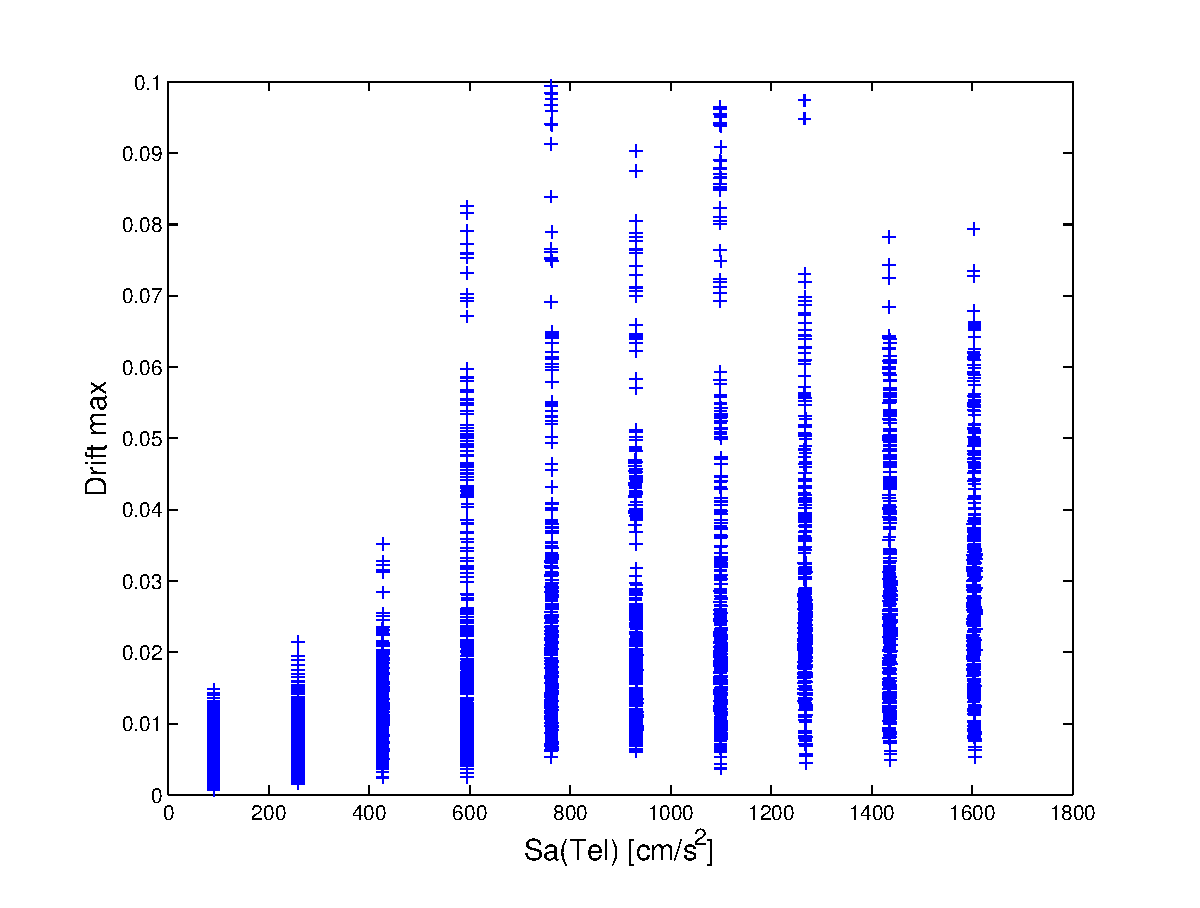
\includegraphics[width=5cm,height=5cm]{./Figures/regression_R3.eps}}
\end{pspicture}

\begin{figure}[H]
\centering
\includegraphics{./figures/PushoverCurve.png}
\caption{Idealised pushover curve.}
\label{fig:expIdealised}
\end{figure}

\item Dynamic parameters of the building: fundamental period of vibration T$_1$ and corresponding modal participation factor $\Gamma_1$.
\item Limit States in terms of roof displacement or inter-storey drift ratio.
\item Consequence function (damage factor for each damage state).
\end{itemize}

\subsection{Options}
\label{sub:options}
The type of procedure to be performed and the type of inputs at disposal, are set with the variables \textit{an\_type} and \textit{in\_type} respectively. With the variable \textit{an\_type} the user can choose between:

\begin{Verbatim}[frame=single, commandchars=\\\{\}, samepage=true]
an\_type = 0 #Cr-based procedure (Ruiz-Garcia and Miranda, 2007)
an\_type = 1 #spo2ida-based procedure (Vamvatsikos and Cornell, 2005)
\end{Verbatim}

With the variable \textit{in\_type} the user can choose between:

\begin{Verbatim}[frame=single, commandchars=\\\{\}, samepage=true]
in\_type = 0 # idealised pushover curve
in\_type = 1 # raw results from a pushover analysis
\end{Verbatim}

The variable \textit{vulnerability} instead gives the opportunity to decide the type of outputs, whether to stop the process at the derivation of the fragility curves, or to go all the way up to the vulnerability curve definition, applying damage-to-loss functions.

\begin{Verbatim}[frame=single, commandchars=\\\{\}, samepage=true]
vulnerability = 0 # derive fragility curves 
vulnerability = 1 # derive vulnerability curve
\end{Verbatim}

The variable \textit{g} serves the purpose of defining the units that are being used. A floating number must be assigned to the gravity acceleration, compatible with the units used for the period of vibration and for the displacements (if the period is expressed in seconds and displacements are in meters, then g = 9.81). The variable \textit{iml} is a numpy array that identifies the intensity measure levels for which loss ratios are computed and provided in the vulnerability curve.

\begin{Verbatim}[frame=single, commandchars=\\\{\}, samepage=true]
g = 9.81
iml = np.linspace(0.1,15,100)
\end{Verbatim}

The variable \textit{plotflag} allows or inhibits the displaying of plots. It is a python list composed of 4 integers, each one controlling a different plot: idealised pushover curve, 16\%-50\%-84\% ida curves, fragility curves and vulnerability curve respectively. Each integer can take as value either zero or one, whether the corresponding graph has to be displayed or not:

\begin{Verbatim}[frame=single, commandchars=\\\{\}, samepage=true]
plotflag = [1, 1, 1, 1] # plot all the graphs
plotflag = [0, 0, 0, 0] # do not plot any graph
\end{Verbatim}

The following variables set some of the characteristics of the plots:

\begin{itemize}
\item \textit{linew}: integer for defining lines width.
\item \textit{fontsize}: fontsize used for labels, graphs etc.
\item \textit{units}: list of 3 strings defining displacements, forces and Spectral acceleration units, as ['[kN]', '[m]', '[m/s$^2$]'], to be displayed on the axes of the plots.
\end{itemize}

The last set of variables is needed for spo2ida-based procedure only:

\begin{itemize}
\item \textit{pw}: floating number assigning pinching level (from 0 to 1)
\item \textit{filletstyle}: integer enabling or not the use of a spline line to link branches of IDA curves

\begin{Verbatim}[frame=single, commandchars=\\\{\}, samepage=true]
filletstyle = 0 # don't use spline curve
filletstyle = 3 # use spline (recommended)
\end{Verbatim}

\item \textit{N}: number of points per segment of IDA curve derived with spo2ida
\item \textit{MC}: number of Monte Carlo simulations to account for uncertainty in damage thresholds
\end{itemize}

\section{C$_R$-based procedure}
\label{sec:CR}
\subsection{Theoretical background}
The aim of this procedure, proposed by Vamvatsikos (2014), is the estimation of the median spectral acceleration value $\hat{s}_c$, that brings the structure to the attainment of a set of damage states, and the corresponding dispersion beta $\beta_{sc}$, the parameters needed for the mathematical representation of fragility in equation \ref{eq:fragility-definition}. The aim is achieved making use of the work by Ruiz-Garcia and Miranda (2007), where the inelastic displacement demand is related to the elastic displacement with a simple relationship, and it can thus be easily estimated through a response spectrum analysis and a capacity curve.

The C$_R$-based procedure presented herein is applicable to bilinear elasto-plastic capacity curve only, and it is suitable for single building fragility curve estimation, as described in section \ref{subsubsec:single-building}. However the fragility curves derived for single buildings can be combined in a unique fragility curve, which considers the inter-building uncertainty, as described in section \ref{subsubsec:multiple-buildings}.

\subsubsection{Single Building Fragility and Vulnerability function}
\label{subsubsec:single-building}
This procedure provides a simple relationship between median damage state threshold, expressed in terms of top displacement $\delta_{roof}$, at each damage state threshold ds, and the corresponding median elastic Spectral displacement value $\hat{S}_{d,ds}(T_1)$.

\begin{equation}
\hat{\delta}_{roof, ds} = C_R S_{d, ds}(T_1) \Gamma_1 \Phi_1
\end{equation}

where $\Gamma_1 \Phi_1$ is the first mode participation factor estimated for the first-mode shape normalised by the roof displacement, and C$_R$ is the inelastic displacement ratio (inelastic over elastic spectral displacement), computed by Ruiz-Garcia and Miranda (2007) for nonlinear SDoF systems having hysteretic behaviour representative of the analysed structure, which is a function of the first-mode period of vibration and the relative lateral strength of the system R. Therefore the median Spectral acceleration at the fundamental period of vibration $\hat{S}_{a,ds}(T_1)$ turns out to be expressed as a function of the roof displacement according to the following equation:

\begin{equation}
\hat{S}_{a,ds}(T_1) = \frac{4 \pi^2}{\hat{C}_R T^2 \Gamma_1 \Phi_1} \hat{\delta}_{roof, ds}
\label{eq:Sa_RGM}
\end{equation}

Default values of $\hat{C}_R$ parameter estimates are provided by Ruiz-Garcia and Miranda (2007), as result of nonlinear regression analysis of three different measures of central tendency computed from 240 ground motions:

\begin{equation}
\hat{C}_R = 1 + \frac{R - 1}{79.12 T_1 ^{1.98}}
\label{eq:Cr_RGM}
\end{equation}

and values for R are given as:

\begin{equation}
R_{ds} = max(0.425(1 - c + \sqrt{c^2 + 2c(2 \mu_{ds} - 1) + 1}),1)
\label{eq:R_RGM}
\end{equation}

where c = 79.12 T$^{1.98}$, and $\mu_{ds}$ is the ductility at the damage state threshold of interest.

For what concerns the dispersion of $\hat{S}_{a,ds}$, $\beta_{sc}$, the following relationship between S and the median EDP damage threshold $\hat{\theta}$ (Cornell, 2002) is used:

\begin{equation}
\hat{\theta}(s) = a S^b
\end{equation}

so that $\beta_{sc}$ can be easily derived from the dispersion of $\theta$ due to record-to-record variability, $\beta_{\theta d}$, as in the following:

\begin{equation}
\beta_{sc} = \frac{1}{b} \beta_{\theta d}
\label{eq:betaSa_RGM}
\end{equation}

The dispersion of $\theta$ due to record-to-record variability, $\beta_{\theta d}$ can be easily combined with the dispersion of $\theta$ due to uncertainty in the damage state threshold $\beta_{\theta c}$ as shown in the following equation:

\begin{equation}
\beta_{sc} = \frac{1}{b} \sqrt{\beta_{\theta d}^2 + \beta_{\theta c}^2}
\label{eq:betaSc_RGM}
\end{equation}

The dispersion of $\theta$ can be obtained assuming that $d_{roof}$ and $\theta$ are proportional, and they thus share the same dispersion. Moreover the dispersion of $d_{roof}$ is the same as the dispersion of C$_R$, since they are also proportional. Finally $\beta_{\theta d}$ can be computed with the following equation, which represents Ruiz-Garcia and Miranda's (2007) estimate of C$_R$ dispersion:

\begin{equation}
\sigma_{\ln(C_R)} = \sigma_{\ln(d_{roof})} = \beta_{\theta d} =  1.975 [\frac{1}{5.876} + \frac{1}{11.749 (T + 0.1)}] [1- \exp(-0.739 (R - 1))]
\end{equation}

To derive a discrete vulnerability function at certain intensity measure levels, the input damage-to-loss factors are applied to the probability of occurance of each damage state, extracted from the probability of exceedance of each damage state described by the fragility function. A value of loss ratio is thus defined for the vector of selected intensity measure levels.

\subsubsection{Multiple-Building Fragility and Vulnerability function}
\label{subsubsec:multiple-buildings}
If multiple buildings have been input to derive fragility curves for a class of buildings all $\mu_{S_a, blg}$ and $\sigma_{S_a, blg}$ are combined in a single lognormal curve. A minimum of 5 buildings should be considered to obtain reliable results for the class. Medians $\hat{S}_{a,ds}$ and total dispersions $\beta_{sc}$ are converted to logarithmic mean $\mu_{S_a}$ and logarithmic standard deviation $\sigma_{S_a}$, according to the following equations:

\begin{equation}
\mu_{S_a} = \hat{S}_a e^{\frac{\beta_{sc}^2}{2}}
\label{eq:median-to-mean}
\end{equation}
\begin{equation}
\sigma_{S_a} = \sqrt[2]{(\beta_{sc}^2-1) e^{2\ln{ \hat{S}_a}+\beta_{sc}^2}}
\label{eq:dispersion-to-standard}
\end{equation}

A new issue arises when multiple buildings are considered: the S$_a$ at the fundamental period of each building should be converted to a common intensity measure, to be able to combine the different fragility functions. A common intensity measure is selected to be S$_a$ at the period T$_{av}$, which is a weighted average of the individual buildings fundamental period T$_1$. Then each individual fragility needs to be expressed in terms of the common S$_a$(T$_{av}$), using a spectrum. FEMA P-695 far field set of 22 accelerograms was used to derive a mean uniform hazard spectrum, and the ratio between the S$_a$ at different periods is used to scale the fragility functions. It can be noted that the actual values of the spectrum are not important, but just the spectral shape. Given the linear transformation, the parameters of the scaled fragility curves of each building are simply:

\begin{equation}
\mu_{S_a, blg} = \mu_{S_a, blg} S(T_{av})/ S(T_{1, blg})
\end{equation}
\begin{equation}
\sigma_{S_a, blg} = \sigma_{S_a, blg} S(T_{av})/ S(T_{1, blg})
\label{eq:Sa(Tav)}
\end{equation}

Finally the parameters of the single lognormal curve for the class of building, logarithmic mean and logarithmic standard deviation, can be computed as the weighted mean of the single means and the SRSS of the inter-building and intra-building standard deviation, the weighted standard deviation of the single means, and the weighted mean of the single standard deviations, respectively, as shown in the following equations:

\begin{equation}
\mu_{S_a, tot} = \sum_{i=0}^{n.blg} w_{blg-i} \mu_{S_a, blg-i}
\label{eq:combination-lognormals-mu}
\end{equation}
\begin{equation}
\sigma_{S_a, tot} = \sqrt{ \sum_{i=0}^{n.blg} w_{blg-i} (\mu_{S_a, blg-i}-\mu_{S_a, tot})^2+(\sum_{i=0}^{n.blg} w_{blg-i} \sigma_{S_a, blg-i})^2}
\label{eq:combination-lognormals-sigma}
\end{equation}

A single vulnerability function can be also obtained, from the single building vulnerability functions. The input damage-to-loss function is applied to the fragility function derived for each building. For the selected intensity measure levels a value of loss ratio is thus defined for each building. Finally a lognormal distribution of the loss ratios is assumed at each iml and the discrete vulnerability function for the entire class of buildings is represented at each iml by the weighted mean and the weighted standard deviation of all the computed loss ratios.

\subsection{Inputs}
\label{subsec:InputCr}
The inputs must be formatted as comma-separated value files (.csv), and saved in the folder \textit{input}, contained in the NSP directory. If any other environment different from Windows is used make sure that the "comma separated values Windows" is selected as saving option when creating the input files. 

If multiple buildings want to be analysed to consider the inter-building uncertainty the parameters relative to each building should be added as additional lines in the input tables, as shown in the examples below, otherwise a single line must be input.

If the user has already at disposal an idealised elasto-plastic pushover curve for each building, that is to say that the variable \textit{in\_type} has been set to 0, the following data need to be provided in the corresponding csv files:

\begin{enumerate}
\item First period of vibration T$_1$, corresponding modal participation factor $\Gamma_1$, normalised with respect to the roof displacement, and weight for the combination of different buildings, input in \textit{building\_parameters.csv}, as in the example below:
	\begin{table}[H]
	\centering
	\begin{tabular}{|c|c|c|c|} \hline
	\textbf{n.building} & \textbf{T$_1$} & \textbf{$\Gamma_1$} & \textbf{weights}\\ \hline
	1 & 0.32 & 1.23 & 0.2\\ \hline
	2 & 0.40 & 1.25 & 0.3\\ \hline
	... & ... & ... & ... \\ \hline
	\end{tabular}
	\end{table}
	
\item Roof displacement at each limit state LS and corresponding dispersion $\beta_{\theta c}$ input in \textit{displacement\_profile.csv}, as shown in the example below. If dispersion is unknown, $\beta_{\theta c}$ can be set equal to zero at each LS.
	\begin{table}[H]
	\centering
	\begin{tabular}{|c|c|c|c|} \hline
	\textbf{n.building} & \textbf{LS$_1$} &	\textbf{LS$_2$} &	\textbf{LS$_3$} \\ \hline
	1 & 0.066 & 0.169 & 0.23\\ \hline
	$\beta_{\theta d, 1}$ & 0.1 & 0.3 & 0.4\\ \hline
	2 & 0.08 & 0.172 & 0.25\\ \hline
	$\beta_{\theta d, 2}$ & 0.1 & 0.3 & 0.4\\ \hline	
	\end{tabular}
	\end{table}
	
\item Idealised pushover curve, input in \textit{idealised\_curve.csv} as shown below. The only required parameters are the yielding displacement $\delta_y$, the ultimate displacement $\delta_u$ and the yielding force F$_y$.

\begin{table}[H]
\centering
\begin{tabular}{|c|c|c|c|} \hline
\textbf{n.building} & \textbf{d$_y$} & \textbf{d$_u$} & \textbf{F$_y$} \\ \hline
1 & 0.09	& 0.3	 & 523\\ \hline
2 & 0.12	& 0.35	 & 400\\ \hline
... & ...	& ... & ...\\ \hline
\end{tabular}
\end{table}

\item Consequence model (loss ratio per each damage state) consistent with the defined set of damage states, input in \textit{consequence.csv}, as in the example below. A single consequence model can be input. This input is needed only if the variable \textit{vulnerability} has been set to 1.	
	\begin{table}[H]
	\centering
	\begin{tabular}{|c|c|c|} \hline
	\textbf{DS$_1$} & \textbf{DS$_2$} & \textbf{DS$_3$} \\ \hline
	0.2	& 0.5	 & 1\\ \hline
	\end{tabular}
	\end{table}
	
\end{enumerate}

If the idealised curve are not available, \textit{in\_type} = 0 can be selected and the displacements vs base shear at each time step results from a pushover analysis can be input instead. The following data need to be provided in the corresponding csv files:

\begin{enumerate}
\item T$_1$ and corresponding $\Gamma_1$, weight for the combination of different buildings, number of storeys and height of each storey, input in \textit{building\_parameters.csv}, as in the example below:
	\begin{table}[H]
	\centering
	\begin{tabular}{|c|c|c|c|c|c|c|c|c|} \hline
	\textbf{n.building} & \textbf{T$_1$} & \textbf{$\Gamma_1$} & \textbf{weights} & \textbf{n.Storey} & \textbf{H$_1$} & \textbf{H$_2$} & ... & \textbf{H$_n$} \\ \hline
	1 & 0.32 & 1.23 & 0.2 & 4 & 3 & 3 & ... & 3 \\ \hline
	2 & 0.40 & 1.25 & 0.3 & 4 & 4 & 2.7 & ... & 2.7 \\ \hline
	... & ... & ... & ... & ... & ... & ... & ... & ... \\ \hline
	\end{tabular}
	\end{table}
	
\item Displacements at each storey, at each incremental step of the pushover analysis, input in \textit{displacements\_pushover.csv}, as in the example below: 
	\begin{table}[H]
	\centering
	\begin{tabular}{|c|c|c|c|c|c|c|} \hline
	\textbf{n.building} & \textbf{n.Storey} & \textbf{Step1} & \textbf{Step 2} & \textbf{Storey 3} & ... & \textbf{Step n}\\ \hline
	1 &	1 & 0.0001 &	0.0005 &	0.001 & ... & 0.01\\ \hline
	   &	2 & 0.0003 &	0.0010 &	0.002 & ... & 0.02\\ \hline
	   &	3 & 0.0004 &	0.0016 &	0.003 & ... & 0.03\\ \hline
	   &	4 & 0.0006 &	0.0021 &	0.004 & ... & 0.04\\ \hline
	2 &	1 & 0.0001 &	0.0005 &	0.001 & ... & 0.01\\ \hline
	   &	2 & 0.0005 &	0.0012 &	0.002 & ... & 0.03\\ \hline
	   &	... & ... &	... &	... & ... & ...\\ \hline
	\end{tabular}
	\end{table}
	
\item Base shear at each incremental step of the pushover analysis input in \textit{reactions\_pushover.csv}, as in the example below:
	\begin{table}[H]
	\centering
	\begin{tabular}{|c|c|c|c|c|c|} \hline
	\textbf{n.building} &	\textbf{Step1} & \textbf{Step 2} & \textbf{Storey 3} & ... & \textbf{Step n} \\ \hline
	1 & 0.35 & 0.69 & 1.04 & ... & 29.12\\ \hline
	2 & 0.45 & 0.78 & 2.05 & ... & 40.00\\ \hline
	... & ... & ... & ... & ... & ...\\ \hline
	\end{tabular}
	\end{table}
	
\item Drift limit state and corresponding dispersion $\beta_{\theta c}$ input in \textit{limits.csv}. If dispersion is unknown, $\beta_{\theta c}$ can be set equal to zero at each limit state.
	\begin{table}[H]
	\centering
	\begin{tabular}{|c|c|c|c|} \hline
	\textbf{n.building} & \textbf{LS$_1$} &	\textbf{LS$_2$} &	\textbf{LS$_3$} \\ \hline
	1 & 0.01 &	0.025 & 0.0337\\ \hline
	$\beta_{\theta d, 1}$ &	0.1 & 0.2 & 0.25\\ \hline
	2 & 0.014 &	0.030 & 0.0430\\ \hline
	$\beta_{\theta d, 2}$ &	0.1 & 0.2 & 0.25\\ \hline
	\end{tabular}
	\end{table}

\item Consequence model (loss ratio per each damage state) consistent with the defined set of damage states, input in \textit{consequence.csv}, as in the example below. A single consequence model can be input. This input is needed only if the variable \textit{vulnerability} has been set to 1.
	\begin{table}[H]
	\centering
	\begin{tabular}{|c|c|c|} \hline
	\textbf{DS$_1$} & \textbf{DS$_2$} & \textbf{DS$_3$} \\ \hline
	0.2	& 0.5	 & 1\\ \hline
	\end{tabular}
	\end{table}
	
\end{enumerate}

\subsection{Calculation Steps}
The overall workflow of C$_R$-based procedure is summarised in this section. The option \textit{an\_type} must be set equal to 0 and the option \textit{in\_type} according to the input at disposal. The corresponding inputs should follow the requirements described in section \ref{subsec:InputCr}. At this point the code proceeds with the following steps:

\begin{enumerate}
\item
\begin{enumerate}
\item If \textit{in\_type} = 0 roof displacement at limit states and idealised pushover are extracted from \textit{displacement\_profile.csv} and \textit{idealised\_curve.csv} respectively.
\item If \textit{in\_type} = 1 results from pushover analysis are extracted from \textit{displacements\_pushover.csv} and \textit{reactions\_pushover.csv}, and drift limit states from \textit{limits.csv}. The idealised 	pushover curve is then derived in the \textit{idealisation} function, where the idealisation process is conducted according to FEMA-440. The elastic stiffness is defined as the 	tangent stiffness passing through the point of the pushover curve where 60\% of the maximum base shear is reached, and the perfectly plastic branch is set at an height equal to 	the maximum base shear. The yielding point is found as the interception between the elastic and the plastic branch.
\end{enumerate}

\item The csv input files are parsed with the function \textit{read\_data} according to the defined options. The parameters essential to the analysis are return together with a graphical visualisation of the inputs if the variable \textit{plotflag}[0] is equal to 1.

\item The parameters extracted are used in the \textit{simplified\_bilinear} function to derive ductility levels $\mu_{ds}$, median spectral acceleration $\hat{S}_{a,ds}$ and the total dispersion $\beta_{sc}$ at each limit state through the following steps:
\begin{itemize}
\item The idealised MDoF system is transformed into an equivalent SDoF system, using $\Gamma_1$.
\item Ductility levels $\mu_{ds}$ corresponding to each damage threshold, are defined.
\item R and C$_R$ are computed, using eq. \ref{eq:R_RGM} and \ref{eq:Cr_RGM} respectively.
\item $\hat{S}_{a,ds}$ and the corresponding dispersion  $\beta_{\theta d}$ are computed using eq. \ref{eq:Sa_RGM} and \ref{eq:betaSa_RGM} respectively.
\item $\beta_{\theta d}$ is combined with dispersion due to uncertainty in the model $\beta_{\theta c}$, if different from zero, to get the total dispersion $\beta_{sc}$, using eq. \ref{eq:betaSc_RGM}.
\item Medians $\hat{S}_{a,ds}$ and total dispersions $\beta_{sc}$ are converted to logarithmic mean $\mu_{S_a}$ and logarithmic standard deviation $\sigma_{S_a}$, according to equations \ref{eq:median-to-mean} and \ref{eq:dispersion-to-standard} respectively.
\item S$_a$(T$_1$) is converted to the intensity measure in common with the rest of the buildings, S$_a$(T$_{av}$), according to eq. \ref{eq:Sa(Tav)}
\end{itemize}

\item Step 3. is repeated for the number of input buildings.

\item
\begin{enumerate}
\item If vulnerability = 0: All $\mu_{S_a, blg}$ and $\sigma_{S_a, blg}$ are combined in a single lognormal curve, whose parameters mean and standard deviation are evaluated according to equations \ref{eq:combination-lognormals-mu} and \ref{eq:combination-lognormals-sigma}. Fragility curves for the class of buildings are displayed if the variable \textit{plotflag}[2] = 1, and logarithmic $\mu$ and $\sigma$ are exported in the \textit{outputs} folder.
\item If vulnerability =1: Vulnerability curves are derived for each fragility function derived at step 4. For the intensity measure levels defined in the variable \textit{iml} a value of loss ratio is thus defined for each building. They are finally combined in a single mean and its standard deviation, equal to the weighted mean and the weighted standard deviation of the loss ratios, assuming a lognormal distribution, as described in section \ref{subsec:InputCr}. Vulnerability curve for the class of buildings is displayed if the variable \textit{plotflag}[3] = 1, and logarithmic $\mu$ and $\sigma$ at each iml are exported in the \textit{outputs} folder.
\end{enumerate}
\end{enumerate}

\section{Spo2ida procedure}
\label{sec:spo2ida}
\subsection{Theoretical background}
The aim of this procedure is the estimation of the median spectral acceleration value $\hat{s}_c$, that brings the structure to the attainment of a set of damage states, and the corresponding dispersion beta $\beta_{sc}$, the parameters needed for the mathematical representation of fragility in equation \ref{eq:fragility-definition}. The aim is achieved making use of the tool spo2ida (Vamvatsikos and Cornell, 2006), where static pushover curves are converted into 16\%, 50\% and 84\% IDA curves, using empirical relationships from a large database of incremental dynamic analysis results, as shown in Figure~\ref{fig:spo2ida}.

\begin{figure}[H]
\centering
\includegraphics[width=12cm,height=8cm]{./figures/spo2ida.jpg}
\caption{spo2ida tool: IDA curves derived from Pushover curve.}
\label{fig:spo2ida}
\end{figure}

The spo2ida-based procedure presented herein is applicable to any kind of multi-linear capacity curve, and it is suitable for single building fragility curve estimation, as described in section \ref{subsubsec:single-building-spo2ida}. However the fragility curves derived for single buildings can be combined in a unique fragility curve, which considers the inter-building uncertainty, as described in section \ref{subsubsec:multiple-building-spo2ida}.

\subsubsection{Single-building Fragility and Vulnerability function}
\label{subsub:single-building-spo2ida}
Given the idealised capacity curve the spo2ida tool uses an implicit R - $\mu$ - T relation to correlate nonlinear displacement, expressed in terms of ductility $\mu$ to the corresponding medians capacity in terms of the parameters R. R is the lateral strength ratio, defined as the ratio between the spectral spectral acceleration S$_a$ and the yielding capacity of the system S$_{ay}$. 

Each branch of the capacity curve, hardening, softening and residual plateau, is converted to a corresponding branch of the three ida curves, using the R - $\mu$ - T relation, which is a function of the hardening stiffness, the softening stiffness and the residual force. These parameters are derived from the idealised pushover capacity expressed in $\mu$-R terms, as well as the ductility levels at the onset of each branch. If some of the branches of the pushover curve are missing because of the seismic behaviour of the system, spo2ida can equally work with bilinear, trilinear and quadrilinear idealisations.

The result of the spo2ida routine is thus a list of ductility levels and corresponding R values at 50\%, 16\% and 84\% percentiles. The distribution of R values at each ductility level, due to the record-to-record variability, is assumed to be lognormal and it can be easily converted to the dispersion of the lognormal distribution with the following equation:

\begin{equation}
\beta_{R(\mu)} = \frac{\ln R(\mu)_{84\%} - \ln R(\mu)_{16\%}}{2}
\label{eq:betaR}
\end{equation} 

Median R and its dispersion at ductility levels corresponding to the damage thresholds can thus be determined, and $\hat{S}_{a,ds}$ can be easily extracted simply multiplying $R_{50\%}(\mu_{ds})$ by the yielding capacity of the system $S_{ay}$, as shown in the following equation:

\begin{equation}
\hat{S}_{a,ds} = R_{50\%}(\mu_{ds}) S_{ay}
\label{eq:SaR}
\end{equation}
\begin{equation}
S_{ay} = \frac{4 \pi^2 \delta_{roof,y}}{g \Gamma_1 T_1^1}
\end{equation}

Since $\hat{R}$ and $\hat{S}_{a}$ are proportional they share the same dispersion.

If dispersion due to uncertainty in the limit state definition $\beta_{\theta c}$ is different from zero it can not be combined directly with the record-to-record dispersion, but a Monte Carlo sampling of the limit state needs to be performed instead. Different values of ductility limit state are sampled from the  lognormal distribution with median the median value of the ductility limit state, and dispersion the input $\beta_{\theta c}$. For each of these ductilities the corresponding R$_{16\%}$-R$_{50\%}$-R$_{84\%}$ are found and converted into $\hat{S}_{a,ds}$ and $\beta_{\theta d}$ according to equation \ref{eq:SaR} and \ref{eq:betaR}. N random S$_a$ corresponding to the N sampled ductility limit states are computed, and their median and the dispersion are estimated. These parameters constitute the median $\hat{S}_{a,ds}$ and the total dispersion $\beta_{total}$ for the considered damage state. The procedure is repeated for each damage state.

To derive a discrete vulnerability function at certain intensity measure levels, the input damage-to-loss factors are applied to the probability of occurance of each damage state, extracted from the probability of exceedance of each damage state described by the set of fragility curves. 

If dispersion due to uncertainty in the limit state is different from zero a vulnerability function is derived for the N sets of sampled ductility limit states. It results in N loss ratios for each defined intensity measure levels. Finally a lognormal distribution of the loss ratios is assumed at each iml and the vulnerability curve is defined at each iml by the mean and the standard deviation of all the computed loss ratios.

\subsubsection{Multiple-Building Fragility and Vulnerability function}
\label{multiple-building-spo2ida}
If multiple buildings have been input to derive a set of fragility curves for a class of buildings all $\mu_{S_a,blg}$ and $\sigma_{S_a,blg}$ are combined in a single lognormal curve for each damage state. A minimum of 5 buildings should be considered to obtain reliable results for the class. The procedure to get $\mu_{S_a,tot}$ and $\sigma_{S_a,tot}$ for the class of building is the same described in section \ref{subsubsec:multiple-buildings}, but the $\mu_{S_a,blg}$ and $\sigma_{S_a,blg}$ are those derived from each sampled set of ductility limit state.

A single vulnerability curve can also be obtained, from the single building vulnerability curves. If no dispersion in the limit state is defined, the method is the same described in section \ref{subsubsec:multiple-buildings}. Otherwise a vulnerability curve is derived for each building as explained in section \ref{subsub:single-building-spo2ida}, considering the sampled set of ductility limit states, that is to say that the mean loss ratio and its standard deviation at each iml, $\mu_{LS,iml,blg}$ and $\sigma_{LS,iml,blg}$ respectively, are found for each building.
Finally the mean loss ratio and its standard deviation, $\mu_{LS,iml}$ and $\sigma_{LS,iml}$, are found for the entire class of buildings as the weighted mean of the single $\mu_{LS,iml,blg}$ and the SRSS of the inter-building and intra-building standard deviation, the weighted standard deviation of the single $\mu_{LS,iml,blg}$, and the weighted mean of the single $\sigma_{LS,iml,blg}$.

\subsection{Inputs}
\label{subsec:InputSpo2ida}
The inputs must be formatted as comma-separated value files (.csv), and saved in the folder \textit{input}, contained in the NSP directory. If any other environment different from Windows is used make sure that the "comma separated values Windows" is selected as saving option when creating the input files. 

If multiple buildings want to be analysed to consider the inter-building uncertainty the parameters relative to each building should be added as additional lines in the tables, as shown in the examples below, otherwise a single line must be input.

If the user has already at disposal an idealised multilinear pushover curve for each building, that is to say that the variable \textit{in\_type} has been set to 0, the following data need to be provided in the corresponding csv files:

\begin{enumerate}
\item First period of vibration $T_1$, corresponding modal participation factor $\Gamma_1$, normalised with respect to the roof displacement, and weight for the combination of different buildings, input in \textit{building\_parameters.csv}, as in section \ref{subsec:InputCr}, input n. 1.
	
\item Top displacement at each damage state threshold and corresponding dispersion $\beta_{\theta c}$ input in \textit{displacement\_profile.csv}, as in section \ref{subsec:InputCr}, input n. 2. 
	
\item Idealised pushover curve, input in \textit{idealised\_curve.csv} as shown below. The parameters needed to describe the idealised pushover curve are: yielding displacement d$_y$, displacement at the onset of degradation d$_s$, displacement at the onset of residual force d$_{min}$, ultimate displacement d$_u$, maximum force F$_{max}$, residual force F$_{min}$. These parameters are represented in Figure~\ref{fig:quadrilinear}.

\begin{figure}[H]
\centering
\includegraphics[width=12cm,height=8cm]{./figures/quadrilinear.jpg}
\caption{Idealisation of capacity curve using multilinear elasto-plastic form.}
\label{fig:quadrilinear}
\end{figure}

\begin{table}[H]
\centering
\begin{tabular}{|c|c|c|c|c|c|c|} \hline
\textbf{n.building} & \textbf{d$_y$} & \textbf{d$_s$} & \textbf{d$_{min}$} & \textbf{d$_u$} & \textbf{F$_{max}$} & \textbf{F$_{min}$} \\ \hline
1 & 0.09	& 0.3	& a & b & 523 & 430\\ \hline
2 & 0.12	& 0.35	 & a & b & 400 & 305\\ \hline	
\end{tabular}
\end{table}

\item Consequence model (loss ratio per each damage state) consistent with the defined set of damage states, input in \textit{consequence.csv}, as in section \ref{subsec:InputCr}, input n. 5.
	
\end{enumerate}

If these data are not available, \textit{in\_type} = 0 can be selected and the "raw" results from a pushover analysis can be input instead. The same data as in section \ref{subsec:InputCr} for \textit{in\_type} = 0 can be input.

\subsection{Calculations}
The overall workflow of spo2ida-based procedure is summarised in this section. The option \textit{an\_type} must be set equal to 1 and the option \textit{in\_type} according to the input at disposal. The corresponding inputs should follow the requirements described in section \ref{subsec:InputSpo2ida}. At this point the code proceeds with the following steps:

\begin{enumerate}
\item 
\begin{enumerate}
\item If \textit{in\_type} = 0, the roof displacement at each limit state and the idealised pushover curve parameters are extracted from \textit{displacement\_profile.csv} and \textit{idealised\_curve.csv} respectively.

\item If \textit{in\_type} = 1 the results from a pushover analysis are extracted from \textit{displacements\_pushover.csv} and \textit{reactions\_pushover.csv} and drift limit states from {limits.csv}. The idealised pushover curve is then derived in the \textit{idealisation} function, where the idealisation process is conducted according to the Gem Analytical Vulnerability Guidelines.	\end{enumerate}

\item The parameters extracted are used to derive ductility levels $\mu_{ds}$, median spectral acceleration $\hat{S}_{a,ds}$ and the total dispersion $\beta_{sc}$ at each damage threshold through the following steps:
\begin{itemize}
\item The idealised MDoF system is transformed into an equivalent SDoF system, using $\Gamma_1$, and SDoF capacity curve is  expressed in terms of $\mu$-R.

\item The variables for spo2ida tool are extracted from the capacity curve and they are used as input to get the 16\%-50\%-84\% ida curves.

\item The ductility levels $\mu_{ds}$ corresponding to each damage threshold are defined, and the corresponding R$_{16\%}$-R$_{50\%}$-R$_{84\%}$ are found in ida outputs.

\item $\hat{S}_{a,ds}$ and the corresponding dispersion $\beta_{\theta d}$ are computed using eq.~\ref{eq:SaR} and eq.~\ref{eq:betaR}, respectively.

\item Medians $\hat{S}_{a,ds}$ and total dispersions $\beta_{sc}$ are converted to logarithmic mean $\mu_{S_a}$ and logarithmic standard deviation $\sigma_{S_a}$, according to equation \ref{eq:median-to-mean} and \ref{eq:dispersion-to-standard}, respectively.

\item S$_a$(T$_1$) is converted to the intensity measure in common with the rest of the buildings, S$_a$(T$_{av}$), according to eq. \ref{eq:Sa(Tav)}.

\item If dispersion due to uncertainty in the limit state $\beta_{\theta c}$ is different from zero different ductility limit states are sampled and corresponding values of $\hat{S}_{a,ds}$ and $\beta_{\theta d}$ are computed, as described in section \ref{subsub:single-building-spo2ida}, but not yet combined together.
\end{itemize}

\item Step 2. is repeated for the number of input buildings.

\item
\begin{enumerate}
\item If vulnerability = 0: All $\hat{S}_{a,ds}$ and $\beta_{\theta d}$ from all the buildings and all the sampled ductility limit states are combined in a single lognormal curve, as described in section \ref{subsub:single-building-spo2ida}. Fragility curves for the class of buildings are displayed if the variable \textit{plotflag}[2] = 1, and logarithmic $\mu$ and $\sigma$ are exported in the \textit{outputs} folder.
\item If vulnerability =1:  For the intensity measure levels defined in the variable \textit{iml} a value of loss ratio is defined for each building and a standard deviation dispersion due to uncertainty in the limit state $\beta_{\theta c}$ is different from zero. They are finally combined in a single mean and standard deviation, equal to the mean of the loss ratios, and a standard deviation, equal to the SRSS of the inter-building and intra-building standard deviation, as described in section \ref{multiple-building-spo2ida}. Vulnerability curve for the class of buildings is displayed if the variable \textit{plotflag}[3] = 1, and logarithmic $\mu$ and $\sigma$ at each iml are exported in the \textit{outputs} folder.
\end{enumerate}

\end{enumerate}

\section{R-$\mu$-T procedure}
\label{sec:DF}
\subsection{Theoretical background}
The aim of this procedure is the estimation of the median spectral acceleration value $\hat{s}_c$, that brings the structure to the attainment of a set of damage states, and the corresponding dispersion beta $\beta_{sc}$, the parameters needed for the mathematical representation of fragility in equation \ref{eq:fragility-definition}. The aim is achieved making use of a R-$\mu$-T relationship, between the reduction factor R, the ductility $\mu$ and period T, which in this case is based on the work of Dolsek and Fajfar (2004).
The R-$\mu$-T-based procedure presented herein is applicable to any kind of multi-linear capacity curve, and it is suitable for single building fragility curve estimation, as described in section \ref{subsubsec:single-building-DF}. However the fragility curves derived for single buildings can be combined in a unique fragility curve, which considers the inter-building uncertainty, as described in section \ref{subsubsec:multiple-building-DF}.

\subsubsection{Single Building Fragility and Vulnerability function}
\label{subsubsec:single-building-DF}

\chapter{Nonlinear Dynamic Method}
	\input{./oqum/RMTK/02-Nonlinear-Dynamic.tex}
% ==============================================================================
% ----------------------------------------------------------------- Bibliography
\bibliographystyle{apalike}
\bibliography{./Bibliography/RMTK.bib}
% ==============================================================================
% ------------------------------------------------------------------- Back Cover
\end{document}
